\subsection{Cерверная часть}

Основными функциями сервера в данном проекте являются контроль за деятельностью пользователей и передача действий от одного игрока другому. Проанализировав правила игры, можно развернуть диаграмму вариантов~использования для сервера, которую в дальнейшем раскроем либо с помощью диаграмм активности, последовательностей и состояний, либо с помощью сценариев.
  
\begin{figure}[htp]
\centering
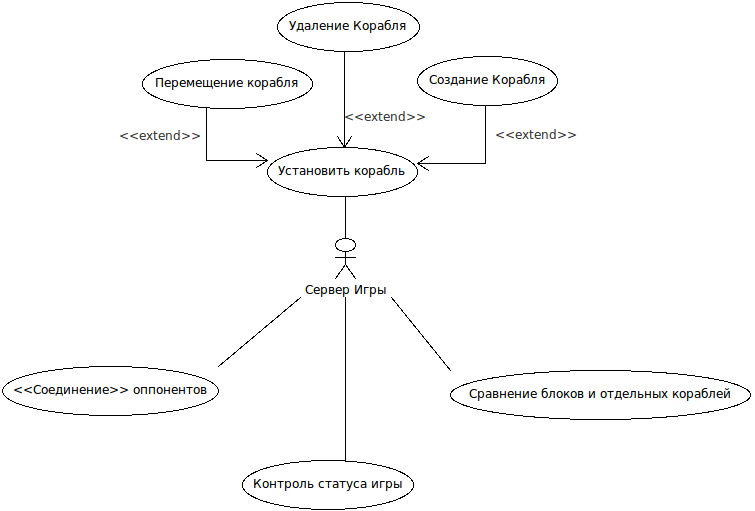
\includegraphics[width=15cm]{images/useserver.png}
\caption{Диаграмма прецедентов сервера}
\label{fig14}
\end{figure}


\begin{figure}[htp]
\centering
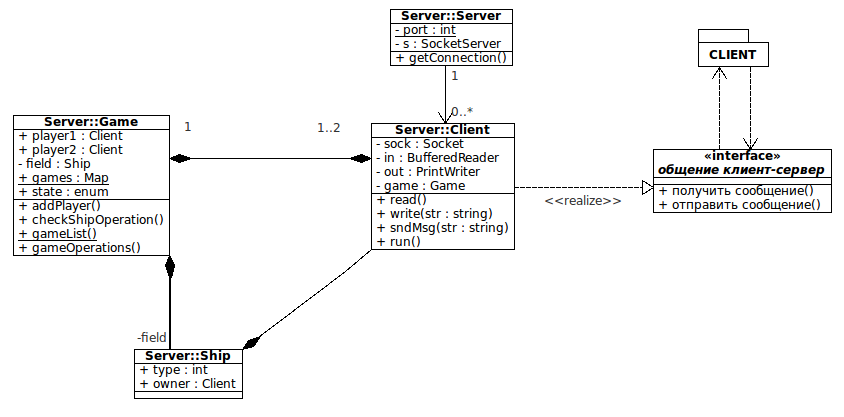
\includegraphics[width=18cm]{images/class_server.png}
\caption{Диаграмма классов сервера}
\label{fig15}
\end{figure}

Класс Ship на диаграмме [\ref{fig15}] используется как вспомогательный класс, фактически как дополнительная структура. Класс Game выполняет те функции, которые были описаны выше, то есть проверяет корректность действий и синхронизирует действия игроков. Именно к классу Game, в основном, будут относиться диаграммы, детализирующие варианты использования.

Обратимся к прецеденту <<Установка кораблей>>. На диаграмме [\ref{fig14}] видно, что он состоит из 3-х частей. Установку и удаление распишем в виде сценариев, а перемещение представим в виде диаграммы состояний [\ref{fig16}].  


\textbf{Создание кораблей:}
	
		\begin{itemize}		
			\item Запрос на создание корабля T от X на клетке [$x,y$];		
			\item Проверить что клетка [$x,y$] свободна;
			\item Проверить, что клетка [$x,y$] на поле игрока X;
			\item Отправить изменения поля обоим игрокам.		
		\end{itemize}


\textbf{Удаление кораблей:}

		\begin{itemize}		
			\item Запрос на удаление корабля T от X на клетке [$x,y$];		
			\item Проверить что клетка [$x,y$] занята кораблем игрока Х;
		\item Отправить изменения поля обоим игрокам.	
		\end{itemize}


\begin{figure}[htp]
\centering
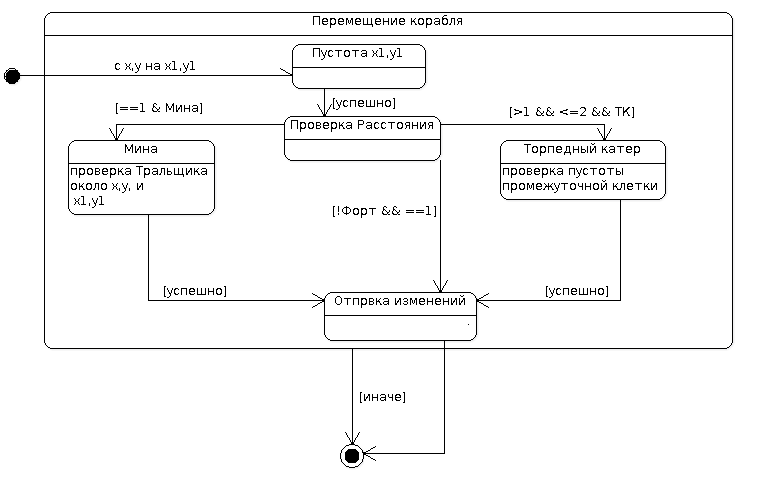
\includegraphics[width=16cm]{images/statemove.png}
\caption{Диаграмма проверки перемещения корабля}
\label{fig16}
\end{figure}

 Отправка изменений должна осуществляться не только оппоненту, но и тому игроку, который совершал ход, так как все действия игроков не отображаются и не фиксируются в клиент-приложении, а осуществляются по командам сервера. Более подробно это описано на примере диаграммы смены статусов игры [\ref{fig17}], изображенной в виде диаграммы последовательностей или в диаграмме [\ref{fig}].

\begin{figure}[htp]
\centering
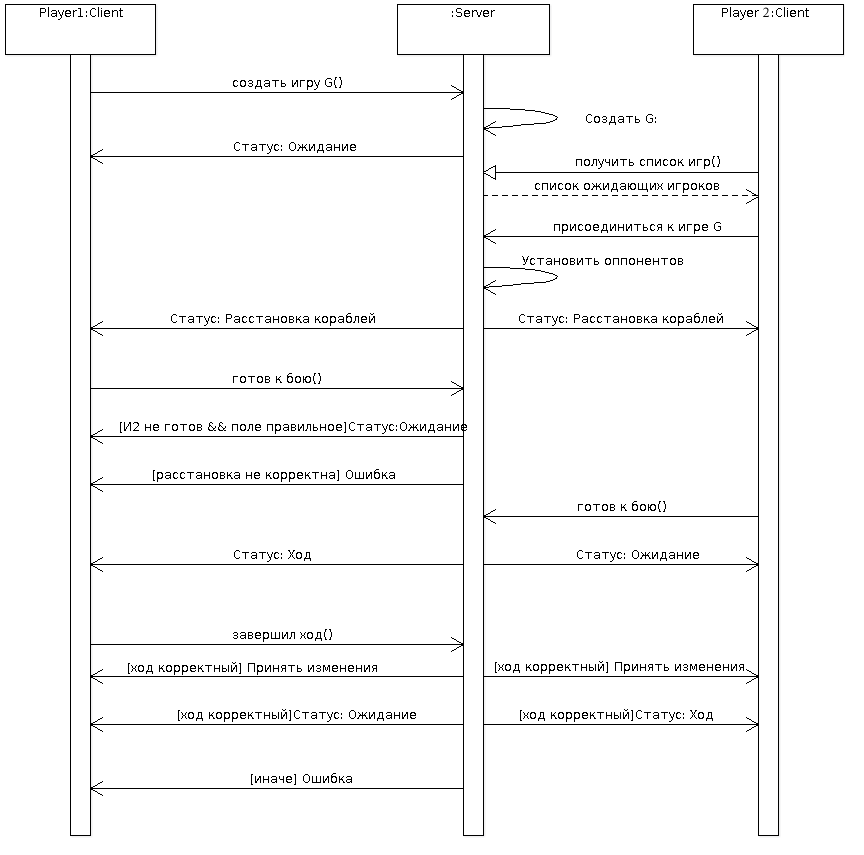
\includegraphics[width=18cm]{images/srvstate.png}
\caption{Диаграмма смены статусов}
\label{fig17}
\end{figure}

В силу равноправности пользователей(т.~е. создателя игры и игрока, который присоединился), диаграмму [\ref{fig17}] можно зеркально отобразить. Этого не было сделано в целях сохранения доступности и понятности схемы. Так же на ней был отмечен статус <<Ход>>, который на самом деле состоит из нескольких подстатусов, таких как: перемещение корабля(является обязательной частью, не подлежащей исключению по правилам), атака корабля противника и, как следствие, ответ противника, взрыв атомной бомбы(только один раз за игру). Последние три действия не являются обязательными для завершения хода. 

Остановимся подробнее на атаке кораблей, то есть рассмотрим прецедент <<Сравнение>>. Этот вариант может быть связан не только с отдельными кораблями, но и с их совокупностью, т. е. блоком.
 Блоком называется объединение двух или трёх кораблей, каждый из которых стоит на соседних клетках по горизонтали или вертикали. Общая схема выполнения сравнения отражена на рисунке [\ref{fig18}], а о мощности блоков и отдельных кораблей подробно написано в источнике [\ref{roganov}].
\begin{figure}[htp]
\centering
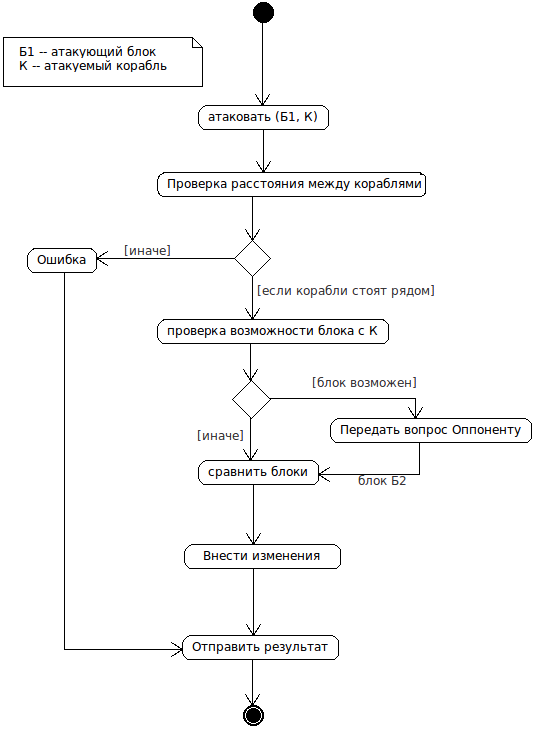
\includegraphics[width=12cm]{images/ask.png}
\caption{Диаграмма сравнения блоков(кораблей)}
\label{fig18}
\end{figure}
\endinput
